\documentclass[letterpaper,12pt]{article}
\usepackage{array}
\usepackage{threeparttable}
\usepackage{geometry}
\usepackage{amsmath}
\geometry{letterpaper,tmargin=1in,bmargin=1in,lmargin=1.25in,rmargin=1.25in}
\usepackage{fancyhdr,lastpage}
\pagestyle{fancy}
\lhead{}
\chead{}
\rhead{}
\lfoot{}
\cfoot{}
\rfoot{\footnotesize\textsl{Page \thepage\ of \pageref{LastPage}}}
\renewcommand\headrulewidth{0pt}
\renewcommand\footrulewidth{0pt}
\usepackage[format=hang,font=normalsize,labelfont=bf]{caption}
\usepackage{listings}
\lstset{frame=single,
  language=Python,
  showstringspaces=false,
  columns=flexible,
  basicstyle={\small\ttfamily},
  numbers=none,
  breaklines=true,
  breakatwhitespace=true
  tabsize=3
}
\usepackage{amsmath}
\usepackage{amssymb}
\usepackage{amsthm}
\usepackage{harvard}
\usepackage{setspace}
\usepackage{float,color}
\usepackage[pdftex]{graphicx}
\usepackage{hyperref}
\hypersetup{colorlinks,linkcolor=red,urlcolor=blue}
\theoremstyle{definition}
\newtheorem{theorem}{Theorem}
\newtheorem{acknowledgement}[theorem]{Acknowledgement}
\newtheorem{algorithm}[theorem]{Algorithm}
\newtheorem{axiom}[theorem]{Axiom}
\newtheorem{case}[theorem]{Case}
\newtheorem{claim}[theorem]{Claim}
\newtheorem{conclusion}[theorem]{Conclusion}
\newtheorem{condition}[theorem]{Condition}
\newtheorem{conjecture}[theorem]{Conjecture}
\newtheorem{corollary}[theorem]{Corollary}
\newtheorem{criterion}[theorem]{Criterion}
\newtheorem{definition}[theorem]{Definition}
\newtheorem{derivation}{Derivation} % Number derivations on their own
\newtheorem{example}[theorem]{Example}
\newtheorem{exercise}[theorem]{Exercise}
\newtheorem{lemma}[theorem]{Lemma}
\newtheorem{notation}[theorem]{Notation}
\newtheorem{problem}[theorem]{Problem}
\newtheorem{proposition}{Proposition} % Number propositions on their own
\newtheorem{remark}[theorem]{Remark}
\newtheorem{solution}[theorem]{Solution}
\newtheorem{summary}[theorem]{Summary}
%\numberwithin{equation}{section}
\bibliographystyle{aer}
\newcommand\ve{\varepsilon}
\newcommand\boldline{\arrayrulewidth{1pt}\hline}


\begin{document}

\begin{flushleft}
  \textbf{\large{Problem Set \#3}} \\
  MACS 30100, Dr. Evans \\
  Soo Wan Kim
\end{flushleft}

\noindent\textbf{Problem 1} \\
\textbf {Part (a)}

\begin{figure}[h!]
  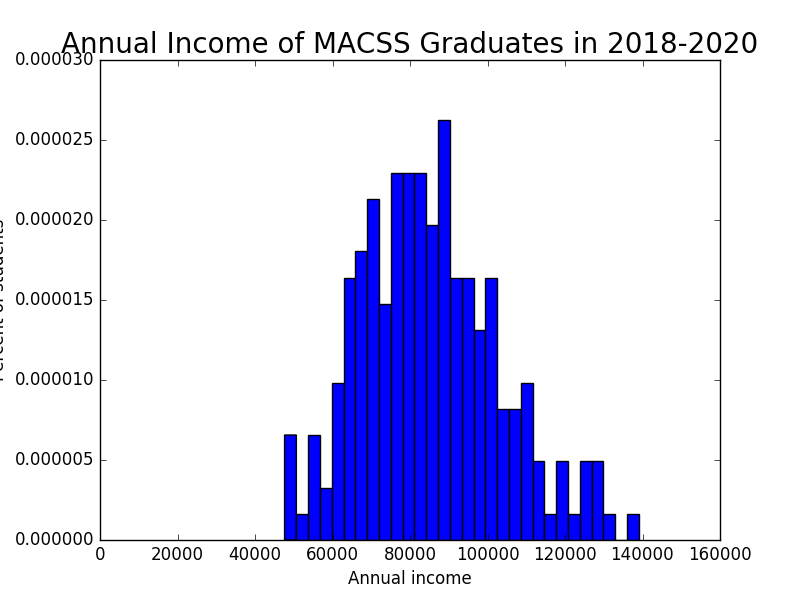
\includegraphics[width=\linewidth]{1a.png}
  \caption{1a: Histogram of percentages of the income.text data}
\end{figure}

\noindent
\textbf {Part (b)} 

\begin{figure}[h!]
  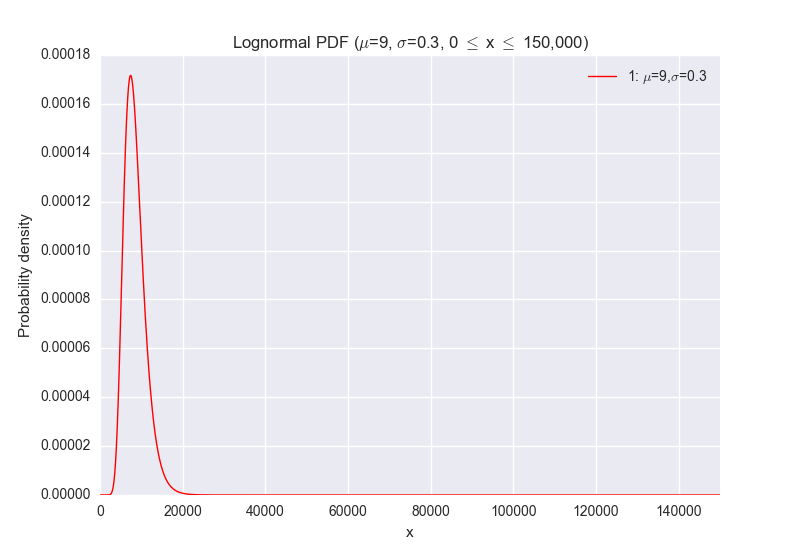
\includegraphics[width=\linewidth]{1b.png}
  \caption{1b}
\end{figure}

\noindent
With the estimated parameter values $\mu$ = 11.3369125379  and $\sigma$ = 0.213026600841, the value of the GMM criterion function is 4.28466184228e-12.\\\\
Data moments and model moments (at the estimated parameter values) compared:\\
Average, standard deviation of income data = (85276.8236063, 17992.542128)\\
Mean, standard deviation of model = (85276.99654884412, 17992.5346699)\\\\
The two sets of values are nearly the same, and as can be seen in figure 2 the model fits the data closely.\\

\noindent\textbf {Part (c).} 

\begin{figure}[h!]
  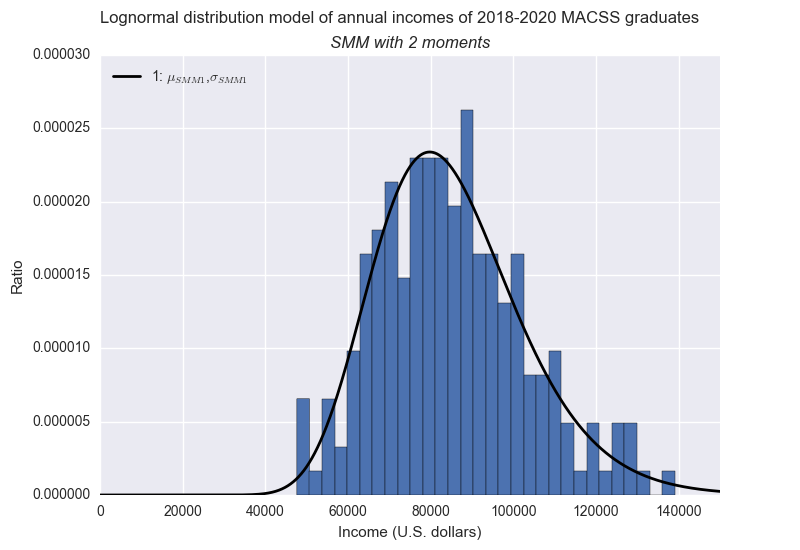
\includegraphics[width=\linewidth]{1c.png}
  \caption{1c}
\end{figure}

\noindent
With the estimated parameter values $\mu$ = 11.3369118806 and $\sigma$ = 0.213028443998, the value of the GMM criterion function is 2.74916504846e-05.\\\\
Data moments and model moments compared:\\
Average, standard deviation of income data = (85276.8236063, 17992.542128)\\
Mean, standard deviation of model (one step estimation) = (85276.99654884412, 17992.5346699)\\
Mean, standard deviation of model (two step estimation) = (85276.9417078091, 17992.6641098)\\\\
The data and model moments are nearly the same for both the one-step and two-step estimations, and again the PDFs are a good fit.\\

\noindent\textbf {Part (d).} \\

\begin{figure}[h!]
  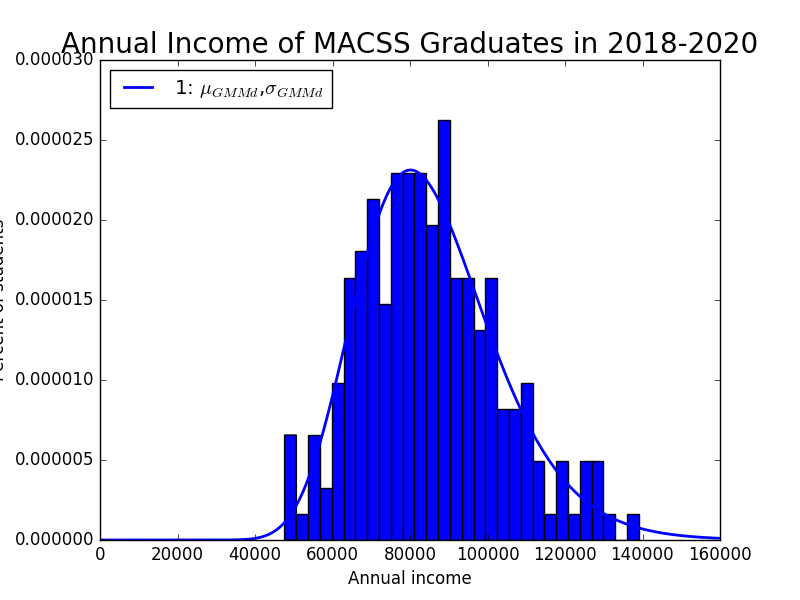
\includegraphics[width=\linewidth]{1d.png}
  \caption{1d}
\end{figure}

\noindent
With the estimated parameter values $\mu$ = 11.3356813175 and $\sigma$ = 0.210598459877, the value of the GMM criterion function is 1.36717737432e-14.\\\\
Data moments and model moments compared:\\
Proportion of individuals earning less than \$75,000, between \$75,000 and \$100,000, and more than \$100,000 respectively: (0.3, 0.5, 0.2)\\
Model moments: (0.30000002529239217, 0.49999999045500304, 0.19999998425260479)\\\\
The data and model moments are almost identical, and the PDF is again a good fit.\\

\noindent
\textbf {Part (e).} \\

\begin{figure}[h!]
  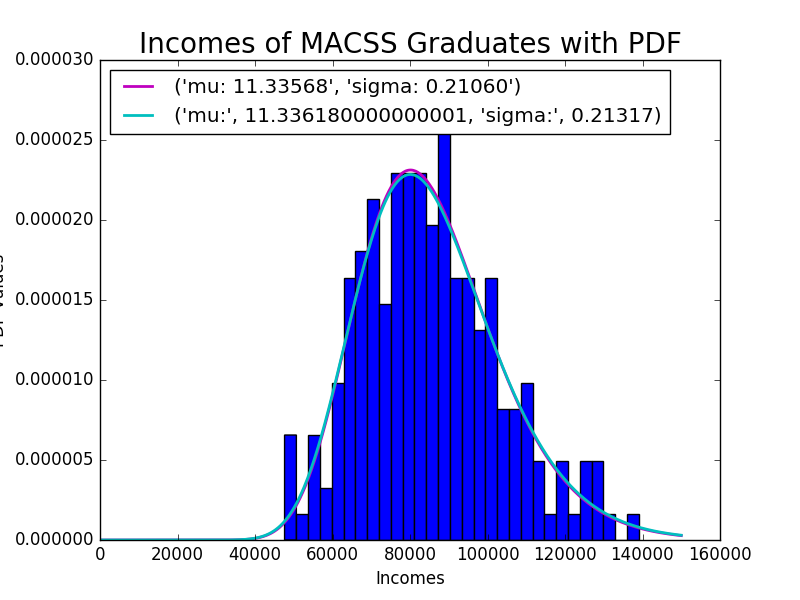
\includegraphics[width=\linewidth]{1e.png}
  \caption{1e}
\end{figure}

\noindent
With the estimated parameter values $\mu$ = 11.3356813261 and $\sigma$ = 0.210598496843, the value of the GMM criterion function is 0.393000895268.\\\\
Data moments and model moments compared:\\
Proportion of individuals earning less than \$75,000, between \$75,000 and \$100,000, and more than \$100,000 respectively: (0.3, 0.5, 0.2)\\
Model moments (one step): (0.30000002529239217, 0.49999999045500304, 0.19999998425260479)\\
Model moments (two step): (0.30000004312708839, 0.49999991985400505, 0.20000003701890656)\\\\
Differences across the data and model moments are very small.\\

\noindent
\textbf {Part (f).} \\

\noindent
The criterion function value is the smallest at the parameterization in part d, which suggests that it fits the data best. However, looking across the figures we can see that all four estimations fit the data closely, with similarly good estimates for the moments chosen. \\\\

\noindent\textbf{Problem 2} \\
\textbf {Part (a).} \\\\
\noindent
Parameter estimates:\\
$\beta_0$ GMM = 0.251645236361\\
$\beta_1$ GMM= 0.0129335385304\\
$\beta_2$ GMM = 0.400500461639\\
$\beta_3$ GMM = -0.00999176023593\\\\
GMM criterion function value = 0.00182128979591

\end{document}
